\section{Methods}\label{sec:methods}

\subsection{Experimental Setup}\label{sec:experimental_method}

The details of the experiments used in obtaining the sorption input data will be discussed i na seaprate paper being prepared on this topic.
Here, we only briefly summarize the experiments.
To study the dynamic sorption of TCE onto the selected building materials, the two-step process shown in Figure \ref{fig:js_sx_setup} was used.\par

A 7.5 by 1.27 cm stainless steel column was filled with a ground sample of the material to be tested.
We use 2.0 g of drywall, and 1.0 g of all the other materials to pack the tube.
Samples were held in by glass wool plugs.
Using flow controllers, TCE was diluted in nitrogen gas to 1.12 $\mathrm{ppb_v}$ and flowed through the column at a rate of 60 mL per minute, for a pre-selected time period.
After the material had been exposed for the selected time, the column was detached and attached to the desorption system.\par

In the desorption system, the sample-containing column was heated to 100 \si{\degreeCelsius} and pure nitrogen gas was flowed through the previously outlet side of the column - carrying the desorbed contaminant with it.
The gas was then passed through a long tube, allowing the gas to cool to room temperature, from which it flowed into a carbon-filled stainless steel sorption column which trapped all of the TCE for analysis.
The sorption column was then desorbed into a gas-chromatograph fitted with a electron capture detector.\par

\begin{figure}
  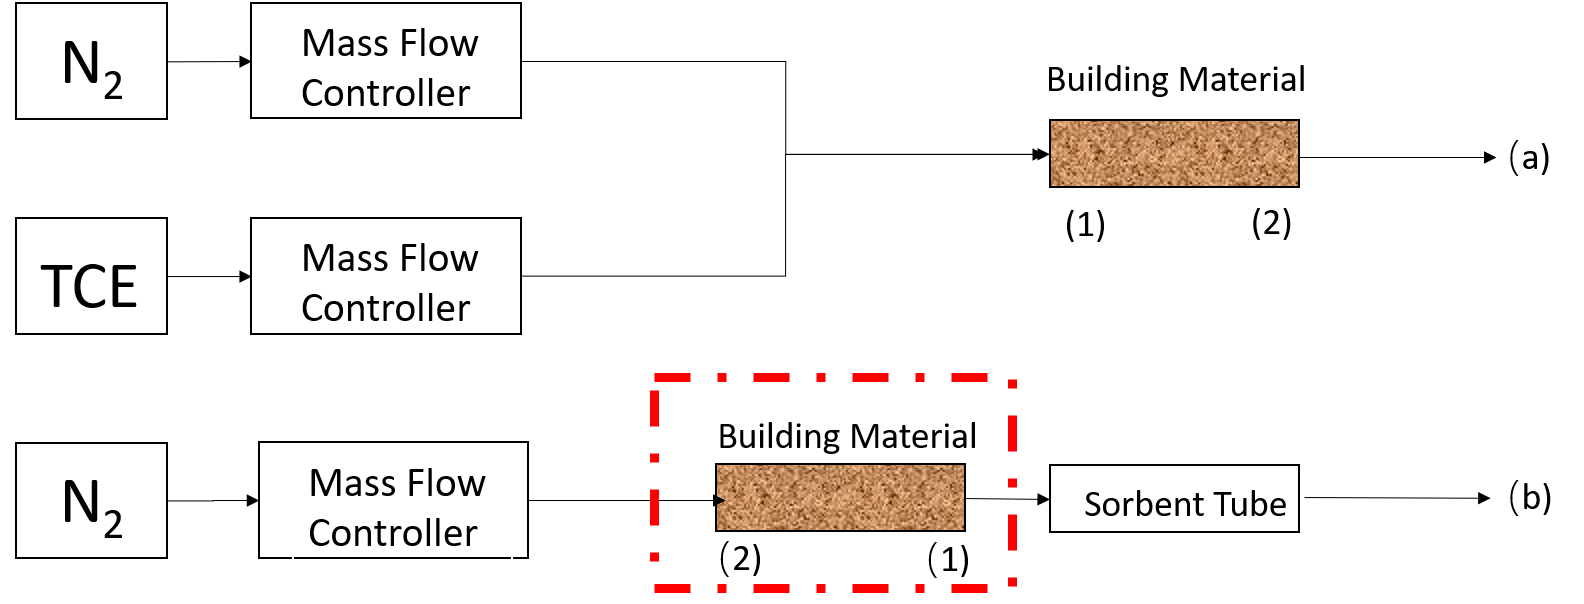
\includegraphics[width=\textwidth]{JS_SX_experiment_setup.png}
  \caption{Schematic of experimental setup.}
  \label{fig:js_sx_setup}
\end{figure}

\subsection{Numerical Model}\label{sec:model}

To investigate the role of sorption in VI, we developed a three-dimensional numerical model of a building overlying a TCE contaminated groundwater source in the commercial finite-element solver COMSOL.
The building is assumed to have a 10 by 10 m footprint, with a 3 meter ceiling height, and its foundation is located 1 m below ground surface (bgs).
The contaminated groundwater is 4 m bgs, and is assumed to be homogenously contaminated with TCE.
The building is surrounded by homogenous soil, that extends 10 m from its walls.
Along the perimeter of the foundation, there is a 1 cm wide crack through which contaminant vapors enter the building and expulsion of contaminant vapors from the indoor occurs through air exchange with the outside.\par

Contaminant vapors are transported from the contaminated groundwater through the soil matrix via advection and diffusion and is described in \ref{sec:mass_transport}.
The presence of the groundwater variably saturates the soil matrix with water, which has a significant effects on the contaminant transport and is modeled using van Genuchten's retention model\cite{van_genuchten_closed-form_1980} and explained in greater detail in section \ref{sec:van_genuchten}.
The water in the soil matrix is assumed to be stationary, thus advective transport only occurs through the vapor phase, while diffusion occurs through both the water and the vapor phases.
The contaminant vapors are also assumed to be able to sorb onto the soil particles, and is modeled using a linear sorption model, and the interaction between the water and vapor phases are determined by Henry's Law.\par

The building is assumed to be pressurized relative to the outside, which gives an air flow in and out of the building (depending on if it is depressurized or overpressurized).
This air flow causes the advective contaminant transport through the soil and the foundation crack.
Darcy's Law is used to model the flow of air and is described in detail in section \ref{sec:darcy}.
A key assumption here is that the contaminant is so diluted in the air, that it is assumed to not affect the transport properties of air.\par

In our implementation, only the soil surrounding the building is explicitly modeled (as a three-dimensional geometry), and the interior of the basement is implicitly modeled as a continuously stirred tank reactor as described in section \ref{sec:indoor_environment}.
These two are coupled via the foundation crack, from which the contaminant entry into the basement is calculated, and contaminant expulsion is determined by the air exchange rate.
In this work we consider the role of sorption on materials in the interior, which is done as a equilibrium reaction.\par

An overview of this modeling approach may be seen in Figure \ref{fig:model}.\par

\begin{figure}
  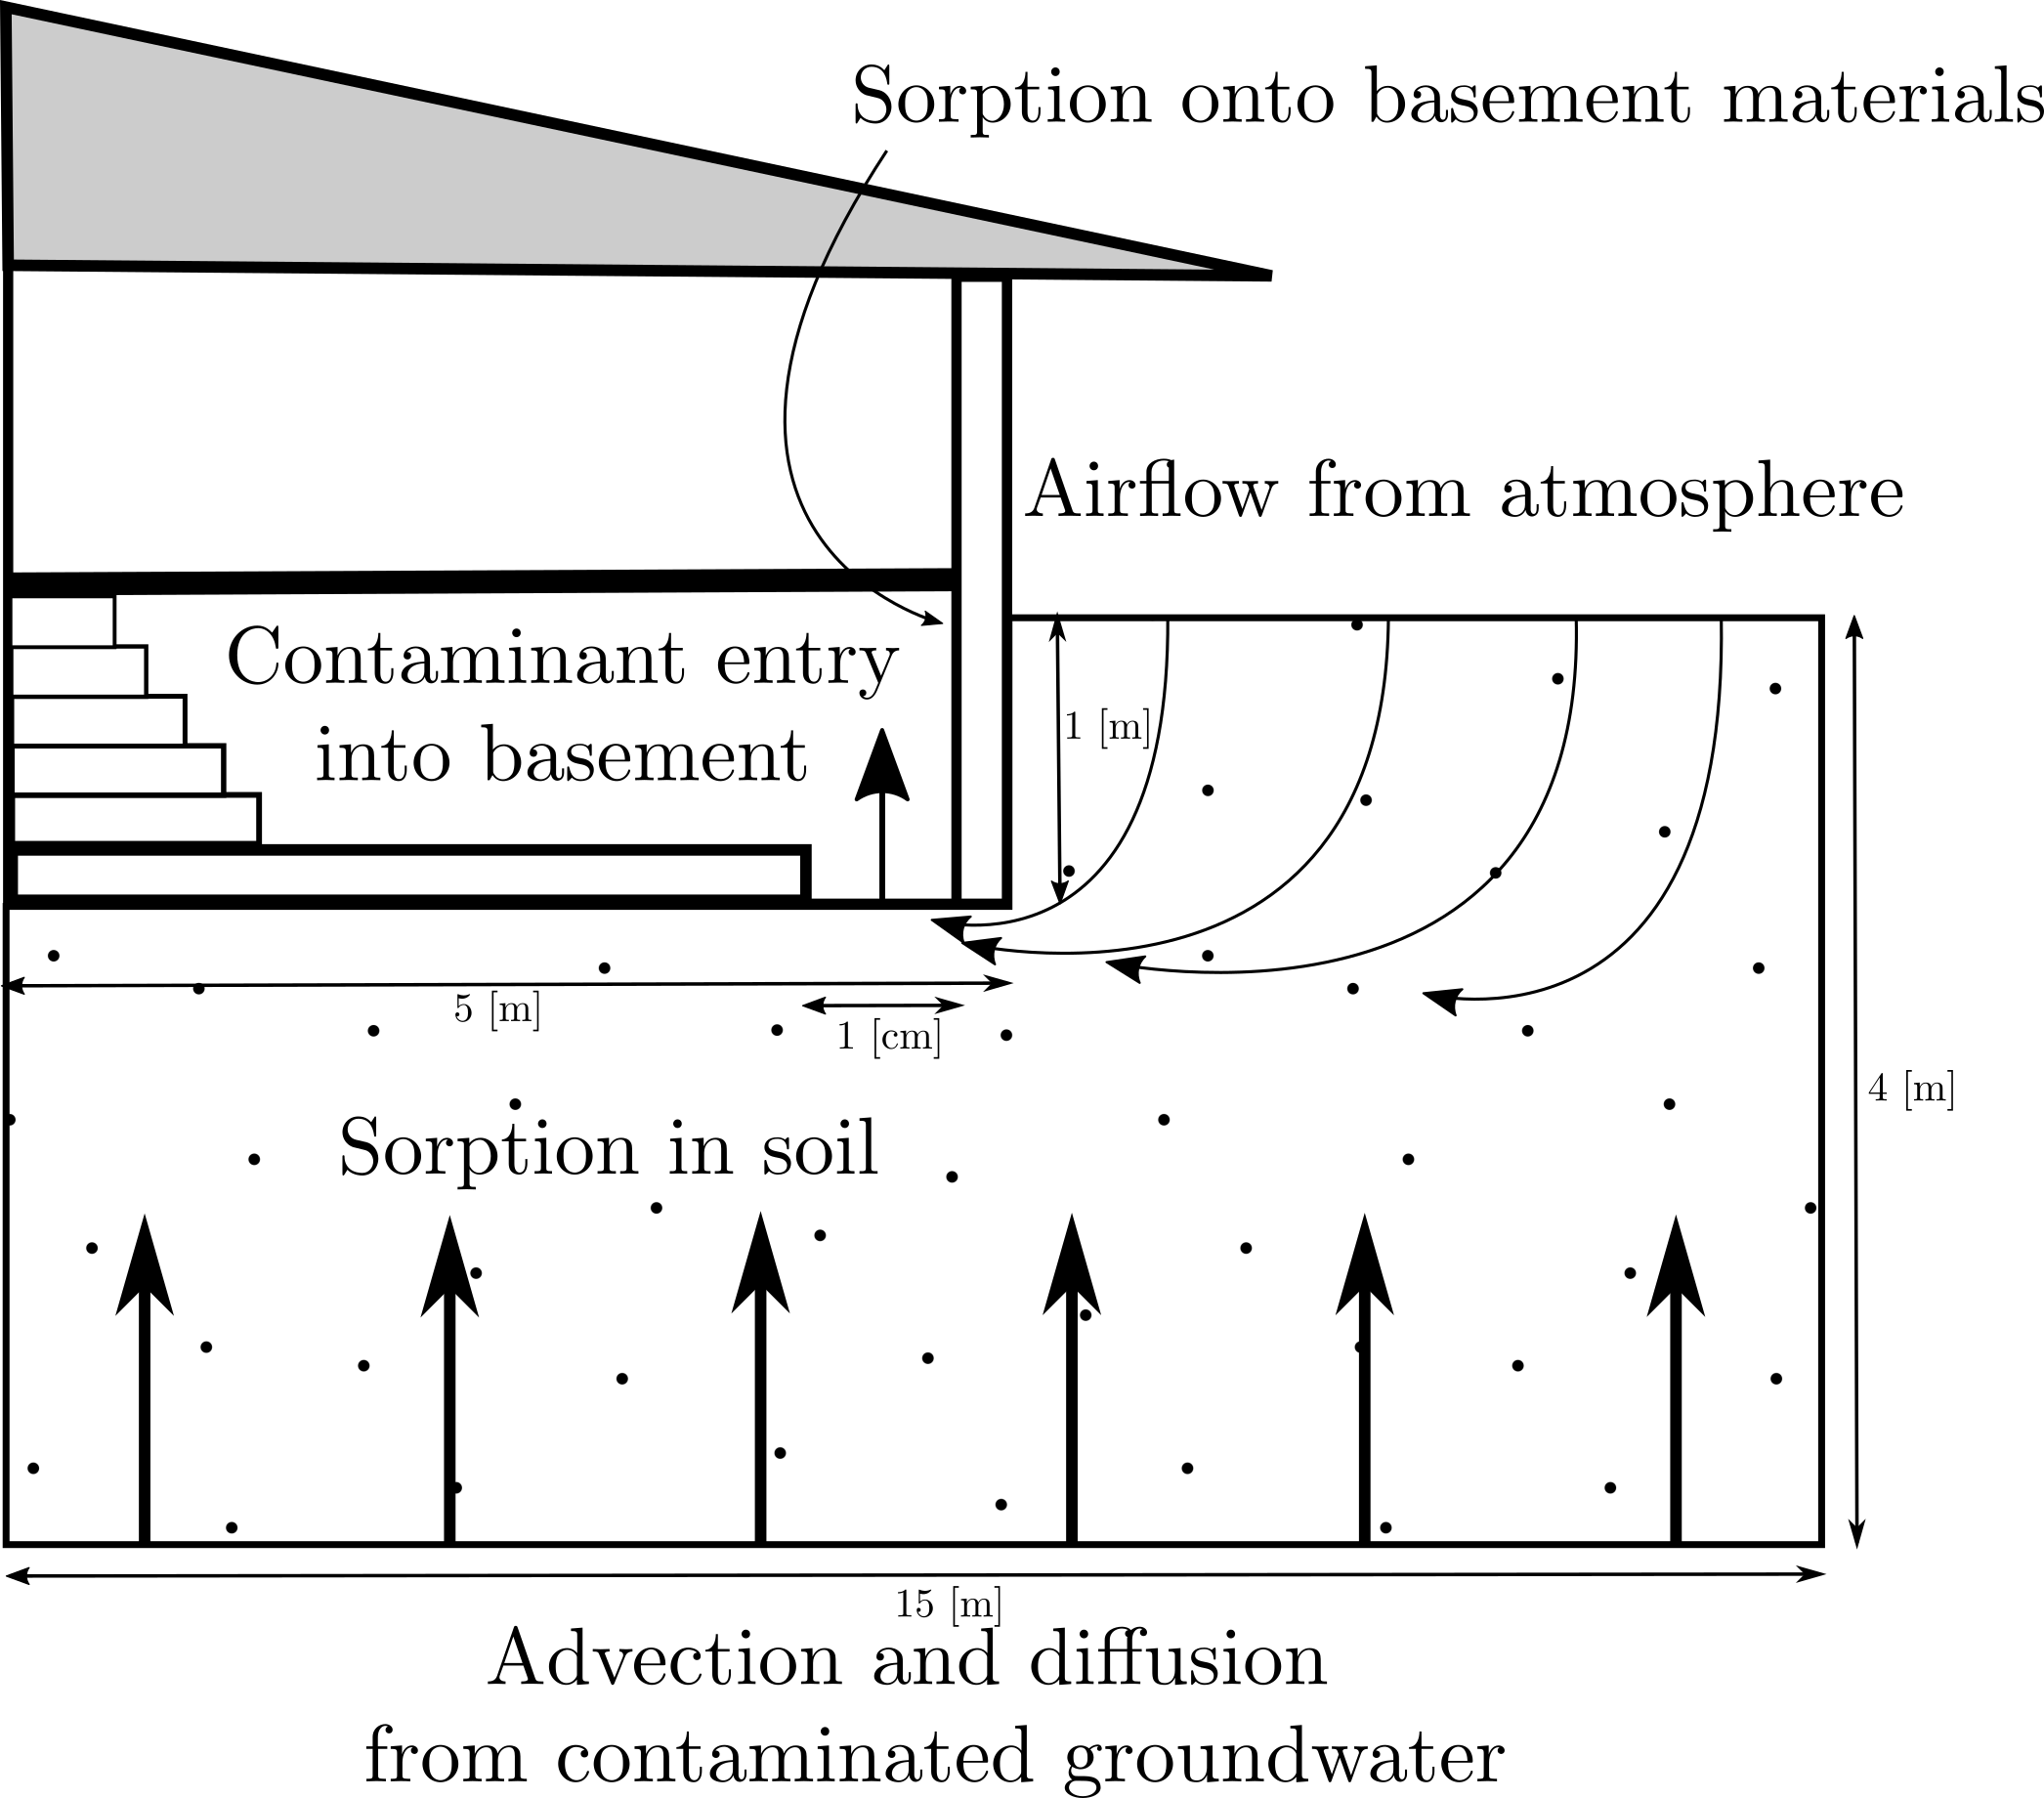
\includegraphics[width=\textwidth]{model.png}
  \caption{Schematic of the modeled vapor intrusion scenario.}
  \label{fig:model}
\end{figure}

\subsubsection{Vadose Zone Moisture Content}\label{sec:van_genuchten}

Since the contaminant transport occurs through the three-phase vadose zone, it is important that we correctly account for soil moisture content and its effect on advective and diffusive transport.
In this modeled scenario, we assume that the soil moisture is at steady-state, and thus the soil moisture content is given by the retention model developed by van Genuchten\cite{van_genuchten_closed-form_1980}.\par

The van Genuchten retention model gives the soil water saturation as a function of elevation above groundwater.
This in turn gives the water and gas filled porosities in the soil, and the relative permeability of the soil matrix.
\begin{align}
  % saturation
  \mathrm{Se} &=
    \begin{cases}\label{eq:van_genuchten_saturation}
      \frac{1}{(1 + \alpha z^n)^m} & z < 0 \\
    1 & z \geq 0
    \end{cases} \\
  % soil moisture
  \theta_w &=
    \begin{cases}\label{eq:van_genuchten_soil_moisture}
      \theta_r + \mathrm{Se}(\theta_s - \theta_r) & z < 0 \\
      \theta_s & z \geq 0
    \end{cases} \\
  % relative permeability
  k_r &=
    \begin{cases}\label{eq:van_genuchten_relative_permeability}
      \mathrm{Se}^l \big[ 1 - \big( 1 - \mathrm{Se}^\frac{1}{m} \big) \big]^2 & z < 0 \\
      0 & z \geq 0
    \end{cases}
\end{align}
$\mathrm{Se}$ is the saturation, and ranges from 0 to 1, which represent completely unsaturated to fully saturated;
$z$ is a height relative to groundwater in meters, with $z=0$ the groundwater surface and $z<0$ into the vadose zone;
$\theta_r$, $\theta_s$, $\theta_w$, and $\theta_g$ are the dimensionless porosity parameters reflecting the residual moisture content, saturated porosity (or just porosity), and water and air filled porosities respectively;
$k_r$ is the relative permeability of water transport and $1-k_r$ gives the relative permeability of air transport.\par

\subsubsection{Gas Flow In The Vadose Zone}\label{sec:darcy}

The gas flow in the vadose zone is governed by a modified version of Darcy's Law.
Originally, Darcy's Law was developed to describe flow in saturated porous media; but flow in unsaturated media requires some modification\cite{c._w._fetter_contaminant_1993}.
An effective permeability that depends on the relative permeability given by the van Genuchten equations is introduced to allow for correct permeability in unsaturated porous media.\par

The vapor flow continuity governing equation is given by
\begin{equation}\label{eq:darcy}
  \frac{\partial}{\partial t} (\rho \theta_s) + \nabla \cdot \rho \Big( -\frac{(1-k_r) \kappa}{\mu} \nabla p \Big) = 0
\end{equation}
Here $\rho$ is the fluid density;
$\kappa$ is the saturated permeability of the soil matrix;
$\mu$ is the fluid viscosity; and $p$ is the fluid pressure.
We assume that the contaminant vapors are so dilute that the gas flow properties can be taken to be those of air, specifically at 20 \si{\degreeCelsius}.
All the transport properties may be found in Table \ref{tbl:model}.\par

\paragraph{Boundary Conditions}

To solve \eqref{eq:darcy} we assign the atmosphere boundary (see Figure \ref{fig:model}) to be the reference pressure, i.e. zero pressure.
The foundation crack boundary is assigned to be at the indoor-outdoor pressure difference value.
Remaining boundaries are no-flow boundary conditions.
\begin{align}
  &\text{Atmosphere} &p = 0 \; \mathrm{(Pa)} \\
  &\text{Foundation crack} &p = p_\mathrm{in} - p_\mathrm{out} = p_\mathrm{in} \; \mathrm{(Pa)} \\
  &\text{All other} &-\vec{n}\cdot\rho\vec{u} = 0 \; \mathrm{(kg/(m^2\cdot s))}
\end{align}
Here $\vec{n}$ and $\vec{u}$ are the boundary normal and gas velocity vectors.

\paragraph{Initial Conditions}

For steady-state problems, the initial conditions do not influence the solution.
Transient simulations however, require initial conditions and these are assumed to be given by the steady-state solution.\par

\subsubsection{Mass Transport In The Vadose Zone}\label{sec:mass_transport}

Contaminants in the vadose zone exist in three phases - gaseous, dissolved in water, and sorbed onto soil particles.
While there are three distinct phase concentrations, the water and gas phases are related via Henry's Law \eqref{eq:henrys_law}.
\begin{equation}\label{eq:henrys_law}
  c_g = K_H c_w
\end{equation}
Where $c_g$ and $c_w$ are the gas and water phase concentrations respectively in $\mathrm{mol/m^3}$;
$K_H$ is the dimensionless Henry's Law constant.\par

In this work, we consider sorption equilibrium between the soil and vapor phases, to be governed by the water contaminant concentration \eqref{eq:linear_sorption}.
\begin{equation}\label{eq:linear_sorption}
  c_s = K_\mathrm{ads} \rho_b c_g = K_\mathrm{ads} \frac{\rho}{1-\theta_s} K_H c_w
\end{equation}
Here the $c_s$ is the solid phase concentration in $\mathrm{mol/kg}$;
$\rho_b$ is the bulk density of the soil $\mathrm{kg/m^3}$, which is given by the density $\rho$ and the total soil porosity $\theta_s$;
$K_\mathrm{ads}$ is the vapor-solid sorption partition coefficient in $\mathrm{m^3/kg}$.\par

Mass transport in the vadose zone is governed by diffusion and advection and is given by \eqref{eq:mass_transport}.
It is important to note that this governing equation is written in terms of the water phase contaminant concentration $c_w$, but via Henry's Law and the vapor-solid sorption partition coefficient, it does in fact describe the contaminant concentration and transport in all three phases.
\begin{equation}\label{eq:mass_transport}
  R \frac{\partial c_w}{\partial t} =
    \nabla \cdot[ D_\mathrm{eff} \nabla c_w] -
    K_H \vec{u} \cdot \nabla c_w
\end{equation}
The first term in \eqref{eq:mass_transport} gives the change in contaminant water concentration with respect to time, modified by the \textit{retardation factor}, $R$, which is discussed below;
The second is the effective diffusive flux which is modified by the effective diffusion coefficient $D_\mathrm{eff}$ which is also discussed below.
The third is the advective flux where $\vec{u}$ is the soil-gas velocity from Darcy's Law, which when multiplied with $K_H$ gives the gas phase concentration advective flux, e.g. advective transport only occurs in the vapor phase and not the liquid phase (the water in the soil matrix is assumed to be at steady-state).\par

\paragraph{Contaminant entry into the building}

The contaminant enters the building through a combination of advection and diffusive fluxes and is given by \eqref{eq:contaminant_entry}.
\begin{equation}\label{eq:contaminant_entry}
  j_{ck} = \begin{cases}
    u_{ck} c_g - \frac{D_\mathrm{air}}{L_\mathrm{slab}} (c_{in} - c_g) & u_{ck} \geq 0 \\
    u_{ck} c_{in} - \frac{D_\mathrm{air}}{L_\mathrm{slab}} (c_{in} - c_g) & u_{ck} < 0
\end{cases}
\end{equation}
Here the $j_{ck}$ is the molar contaminant flux into the building in $\mathrm{mol/(m^2 \cdot s)}$;
$D_\mathrm{air}$ is the contaminant diffusion coefficient in pure air in $\mathrm{m^2/s}$;
$L_\mathrm{slab}$ is the thickness of the foundation slab in $\mathrm{m}$.
The flux expression changes if there is a bulk flow into the building, i.e. $u_{ck} \geq 0$, or out of the building.

\paragraph{Retardation factor}

As the contaminants are transported through the vadose zone, the partitioning between the various phases increases the contaminant residency time, retarding the transport of contaminants.
This effect is represented by $R$ which is the retardation factor \eqref{eq:retardation_factor}.
\begin{equation}\label{eq:retardation_factor}
  R = \theta_w + \theta_g K_H + \rho_b K_H K_\mathrm{ads}
\end{equation}
Here $\theta_w$, $\theta_g$ are the water and gas filled soil porosities;
$K_\mathrm{ads}$ is the vapor-solid partition coefficient in $\mathrm{m^3/kg}$.\par

\paragraph{Effective diffusivity}

The effective diffusivity in the vadose zone varies with the soil moisture content, from being close to that in water when fully saturated and close to that in air when soil moisture is low.
Millington-Quirk developed \eqref{eq:millington-quirk} which describes the effective diffusivity in variably saturated porous media.
\begin{equation}\label{eq:millington-quirk}
  D_\mathrm{eff} = D_\mathrm{water} \frac{\theta_w^\frac{7}{3}}{\theta_s^2} + \frac{D_\mathrm{air}}{K_H} \frac{\theta_g^\frac{7}{3}}{\theta_s^2}
\end{equation}
Where the porosity terms reflect the water and gas phase tortuosity;
$D_\mathrm{air}$ and $D_\mathrm{water}$ are the contaminant diffusion coefficient in air and water respectively in $\mathrm{m^2/s}$;
The Henry's Law constant $K_H$ appears here to reflect that all the contaminant transport is a function of the contaminant water concentration.\par

\paragraph{Boundary Conditions}

In this model, the sole contaminant source is assumed to be the homogenously contaminated groundwater, which we assume to have a fixed concentration.
The atmosphere acts as a contaminant sink and thus this is simply a zero concentration boundary condition.
Contaminants leave the soil domain and enter the building through a combination of advective and diffusive gas phase transport.
The boundary condition applied to all other boundaries is a no-flow boundary.
\begin{align}
  &\text{Atmosphere} & c_w = 0 \; \mathrm{(mol/m^3)} \\
  &\text{Groundwater} & c_w = c_{gw} \; \mathrm{(mol/m^3)} \\
  &\text{Foundation crack} & -\vec{n} \cdot \vec{N} = - \frac{j_{ck}}{K_H} \; \mathrm{(mol/(m^2 \cdot s))}\\
  &\text{All other} & -\vec{n} \cdot \vec{N} = 0 \; \mathrm{(mol/(m^2 \cdot s))}
\end{align}
$\vec{n} \cdot \vec{N}$ is the dot product between the boundary normal vector and the contaminant flux;
$j_ck$ is the contaminant vapor flux into the building.
We assume that only contaminants in the gas phase enter the building, and dividing $j_{ck}$ by $K_H$ we get proper accounting in terms of the water phase concentration accounting in the main transport equation \ref{eq:mass_transport}.\par

\paragraph{Initial Conditions}

For transient simulations in this work, the steady-state solution to a corresponding case is always used as an initial condition.

\subsubsection{Indoor Environment}\label{sec:indoor_environment}

The indoor air space is modeled as a continuously stirred tank reactor (CSTR) given by \eqref{eq:cstr}.
Contaminants are assumed to only enter through the foundation crack, represented by $n_\mathrm{ck}$, which is calculated by integrating the contaminant flux over the foundation crack boundary.
The product of air exchange rate, (which governs how many house volumes are exchanged with the outside per time unit,) and indoor air contaminant concentration gives the contaminant exit rate fromthe house.
The sorption of contaminant on indoor materials is given by the sorption term in \eqref{eq:sorption_rate} and the sorbed contaminant concentration on all interior surfaces is given by \eqref{eq:sorbed_concentration}.

\begin{align}
  V_\mathrm{bldg} \frac{\partial c_\mathrm{in}}{\partial t} &= n_\mathrm{ck} - A_e c_\mathrm{in} V_\mathrm{bldg} - r_\mathrm{sorb} V_\mathrm{mat}\label{eq:cstr} \\
  V_\mathrm{mat} \frac{\partial c_\mathrm{sorb}}{\partial t} &= r_\mathrm{sorb} V_\mathrm{mat}\label{eq:sorbed_concentration} \\
  r_\mathrm{sorb} &= k_1 c_\mathrm{in} - k_2 c_\mathrm{sorb}\label{eq:sorption_rate}\\
  n_\mathrm{ck} &= \int_{A_{ck}} j_{ck} dA
\end{align}

Here $V_\mathrm{bldg}$ and $V_\mathrm{mat}$ are the indoor control volume and volume of indoor material in $\mathrm{m^3}$;
$c_\mathrm{in}$ and $c_\mathrm{sorb}$ are the indoor and sorbed (onto the indoor material) contaminant concentrations in $\mathrm{mol/m^3}$;
$n_\mathrm{ck}$ is the contaminant entry rate in $\mathrm{mol/s}$, which is calculated by integrating the contaminant flux $j_{ck}$ over the foundation crack area;
$r_\mathrm{sorb}$ sorption rate in $\mathrm{mol/(m^3 \cdot s)}$;
$k_1$ and $k_2$ are the sorption and desorption rate constants in $\mathrm{1/s}$.\par

\paragraph{Fitting Kinetic Parameters}

These values of $k_1$ and $k_2$ are found by applying \eqref{eq:sorption_rate} numerically to the experimental data via least square fitting.
We use Runge-Kutta method of order 5(4) as the numerical solve, which is implemented together with the least square method in the SciPy python package\cite{jones_scipy_2011}.


\begin{table}[htb!]
  \setlength{\tabcolsep}{1pt}
  \centering
  \begin{tabular}{l c c c c c c c}
    \toprule
    %%%%%%%%%%%%%%%%%%%%%%%%%%%%%%%%%%%%%%%%%%%%%%%%%%%%%%%%%%%%%%%%%%%%%%%%%%%%
    % SOIL PROPERTIES
    %%%%%%%%%%%%%%%%%%%%%%%%%%%%%%%%%%%%%%%%%%%%%%%%%%%%%%%%%%%%%%%%%%%%%%%%%%%%
    \multicolumn{7}{c}{\textbf{Soil Properties}\cite{abreu_conceptual_2012,u.s._environmental_protection_agency_userss_2004}} \\
    \midrule
    \textbf{Soil} & \textbf{$\kappa \; \mathrm{(m^2)}$} & \textbf{$\theta_s$} & \textbf{$\theta_r$} & \textbf{$\alpha \; \mathrm{(1/m)}$} & \textbf{$n$} & \textbf{$\rho \; \mathrm{kg/m^3}$} \\
    % GRAVEL
    Sand & $9.9 \cdot 10^{-12}$ & 0.38 & 0.053 & 3.5 & 3.2 & 1460 \\
    % SANDY LOAM
    Sandy Loam & $5.9 \cdot 10^{-13}$ & 0.39 & 0.039 & 2.7 & 1.4 & 1460 \\
    %%%%%%%%%%%%%%%%%%%%%%%%%%%%%%%%%%%%%%%%%%%%%%%%%%%%%%%%%%%%%%%%%%%%%%%%%%%%
    % TCE PROPERTIES
    %%%%%%%%%%%%%%%%%%%%%%%%%%%%%%%%%%%%%%%%%%%%%%%%%%%%%%%%%%%%%%%%%%%%%%%%%%%%
    \midrule
    \multicolumn{7}{c}{\textbf{Trichloroethylene (diluted in air) Properties}\cite{abreu_conceptual_2012,u.s._environmental_protection_agency_userss_2004}} \\
    \midrule
    \multicolumn{1}{c}{\textbf{$D_\mathrm{air} \; \mathrm{(m^2/h)}$}} & \textbf{$D_\mathrm{water} \; \mathrm{(m^2/h)}$} & \textbf{$\rho \; \mathrm{(kg/m^3)}$} & \textbf{$\mu \; \mathrm{(Pa \cdot s)}$} & \textbf{$K_H$} \\
    \multicolumn{1}{c}{$2.47 \cdot 10^{-2}$} & $3.67 \cdot 10^{-6}$ & 1.614 & $1.86 \cdot 10^{-5}$ & 0.403 \\
    %%%%%%%%%%%%%%%%%%%%%%%%%%%%%%%%%%%%%%%%%%%%%%%%%%%%%%%%%%%%%%%%%%%%%%%%%%%%
    % BUILDING PROPERTIES
    %%%%%%%%%%%%%%%%%%%%%%%%%%%%%%%%%%%%%%%%%%%%%%%%%%%%%%%%%%%%%%%%%%%%%%%%%%%%
    \midrule
    \multicolumn{7}{c}{\textbf{Building Properties}} \\
    \midrule
    \multicolumn{1}{c}{\textbf{$V_\mathrm{bldg} \; \mathrm{(m^3)}$}} & \textbf{$L_\mathrm{slab} \; \mathrm{(cm)}$} & \textbf{$A_e \; \mathrm{(1/hr)}$} \\
    \multicolumn{1}{c}{300} & 15 & 0.5 \\
    \bottomrule
  \end{tabular}
  \caption{Transport and material properties used in the model. See Table \ref{tbl:abbreviations} for nomenclature.}\label{tbl:model}
\end{table}
